\section{Development View}

Im Folgenden wird die Sicht auf die Anwendung während der Entwicklung beschrieben.

\subsection{Source code organization}
Für die Organisation unseres Quellcodes haben wir einen Monorepo-Ansatz verwendet. Alle Backend-Services, das Frontend und die Dateien für CI/CD sind in diesem Repository in der Ordnerstruktur wie in Figure \ref{fig:repo-structure} gezeigt abgelegt.

\begin{figure}[ht]
    \begin{verbatim}
        park
        |-- backend
        |   |-- authentication
        |   |   |-- ...
        |   |-- infrastructure-administration
        |   |   |-- ...
        |   |-- parking-management
        |   |   |-- ...
        |   |-- property-management
        |   |   |-- ...
        |   |-- shared
        |-- certs
        |-- ci-cd
        |   |-- helm
        |   |   |-- ...
        |   |-- terraform
        |       |-- ...
        |-- cloud-functions
        |-- docs
        |   |-- ...
        |-- frontend
        |   |-- ...
        |-- shared
        |-- signup-frontend
        |-- ...
    \end{verbatim}
    \caption{Repository Structure}
    \label{fig:repo-structure}
\end{figure}

Für alle einzelnen Backend Microservices existiert unter \verb|backend| ein Unterordner, in dem das Node.js Projekt des entsprechenden Microservices abgelegt ist. Zusätzlich sind unter \verb|shared| TypeScript files abgelegt, die von mehreren Backend Services verwendet werden.

Der Ordner \verb|certs| ist für das lokale Testing, um dort die Key-Files der Service Accounts abzulegen.

In \verb|ci-cd| sind alle Dateien für DevOps und das Deployen der Infrastruktur abgelegt. Unter \verb|helm| liegen dabei alle Dateien, die für das Erstellen der Helm Charts benötigt werden, \verb|terraform| beinhaltet alle Konfigurationsdateien für die Cloud-Infrastruktur. Außerdem befinden noch Python-Skripte für das Deployment-Handling in diesem Verzeichnis.

Damit auch der Code für die Cloud-Functions in die Quellcodeverwaltung aufgenommen sind, existiert für diese das \verb|cloud-functions| Verzeichnis.
Unter \verb|docs| liegen einige Files für die Dokumentation ab. Darunter Skizzen für die API-Spezifikation.

Im \verb|frontend| Verzeichnis befindet sich der gesamte Client-Code der Anwendung, in diese Fall ein React Projekt mit allen Komponenten und Services des Frontends.
Außerdem existiert noch ein weiteres \verb|shared| Verzeichnis auf top-level Ebene für die DTOs zwischen Frontend und Backend.

Für die Tenant-Creation, beziehungsweise der Registrierung und Instanzerstellung für neue Tenants existiert noch ein separater Client, welcher unter \verb|signup-frontend| abgelegt ist. Hierbei handelt es sich ebenfalls um ein React-Projekt.

Während der Entwicklung haben wir mit Feature-Branches angelegt an den Git Flow gearbeitet, um eine möglichst konfliktfreie, parallele Entwicklung der Anwendung zu ermöglichen.

\subsection{Components}
Die Applikation umfasst 4 Microservices für das Backend:

\begin{itemize}
    \item \textbf{Authentication Service:} Erweiterung der Authentication-Funktionalität für den Kontext der Anwendung
    \item \textbf{Infrastructure Management Service:} Zentrale Verwaltung der Tenant Creation und Endpunkt zur Konsolidierung von Anwendungsweiten Analytics
    \item \textbf{Parking Management Service:} Bereitstellung der gesamten Funktionalität für das Parken, Laden und die Belegungsverwaltung
    \item \textbf{Property Management Service:} Bereitstellung der Gesamten Funktionalität für die Verwaltung der Parkinfrastruktur
\end{itemize}

Zusätzlich werden 2 Frontend Clients bereitgestellt:

\begin{itemize}
    \item \textbf{PARK Client:} Frontend für die Bedienung der Anwendung
    \item \textbf{SignUp Client:} Frontend für die Tenant-Creation/Instanzerstellung
\end{itemize}

Wie bereits im Kontextdiagram (Figure \ref{fig:context-diagram}) gezeigt, sind zudem verschiedene externe Komponenten angebunden. So werden beispielsweise unterschiedliche Komponenten aus der Google Cloud Infrastruktur verwendet (Object Storage, Firestore, Identity Platform,...). Außerdem werden extern verwaltete Komponenten angebunden, beispielsweise in Form von Schranken, Ladestationen usw. Für das automatisierte Deployment werden GitHub Actions verwendet.

\subsection{Libraries}
Für die Interaktion mit der Google Cloud Infrastruktur wurden unterschiedliche Libraries verwendet. Für den Zugriff auf die Firestore Infrastruktur haben wir das NPM Paket \href{hhttps://www.npmjs.com/package/firebase-admin}{firebase-admin} verwendet, welches verschiedene Methoden, beispielsweise zum Abrufen und Erstellen von Dokumenten in einer Firestore Datenbank zur Verfügung stellt.

Um Zugriff auf den Object Storage zu haben, um beispielsweise bei der Defect-Erstellung Bilder ablegen zu können haben wir den \href{https://www.npmjs.com/package/@google-cloud/storage}{google-cloud/storage} NPM Client verwendet.

Die Kommunikation mit der Google Cloud Identity Platform für das frontendseitige Anmelden ist über das \href{https://www.npmjs.com/package/@firebase/app-compat}{@firebase/app-compat package} realisiert.

Da für die Authentifizierung der Komponenten innerhalb der Anwendung JWT Tokens verwendet werden, sind außerdem die \href{https://www.npmjs.com/package/jsonwebtoken}{jsonwebtoken} Library und der OAuth2Client Client aus der \href{https://www.npmjs.com/package/google-auth-library}{google-auth-library} eingebunden.

\subsection{APIs}
Im Wesentlichen stellt jeder Service eine API bereit, wie in Abbildung \ref{fig:api-overview} dargestellt, über welche dessen Funktionalität genutzt werden kann.

\begin{figure}[ht]
    \centering
    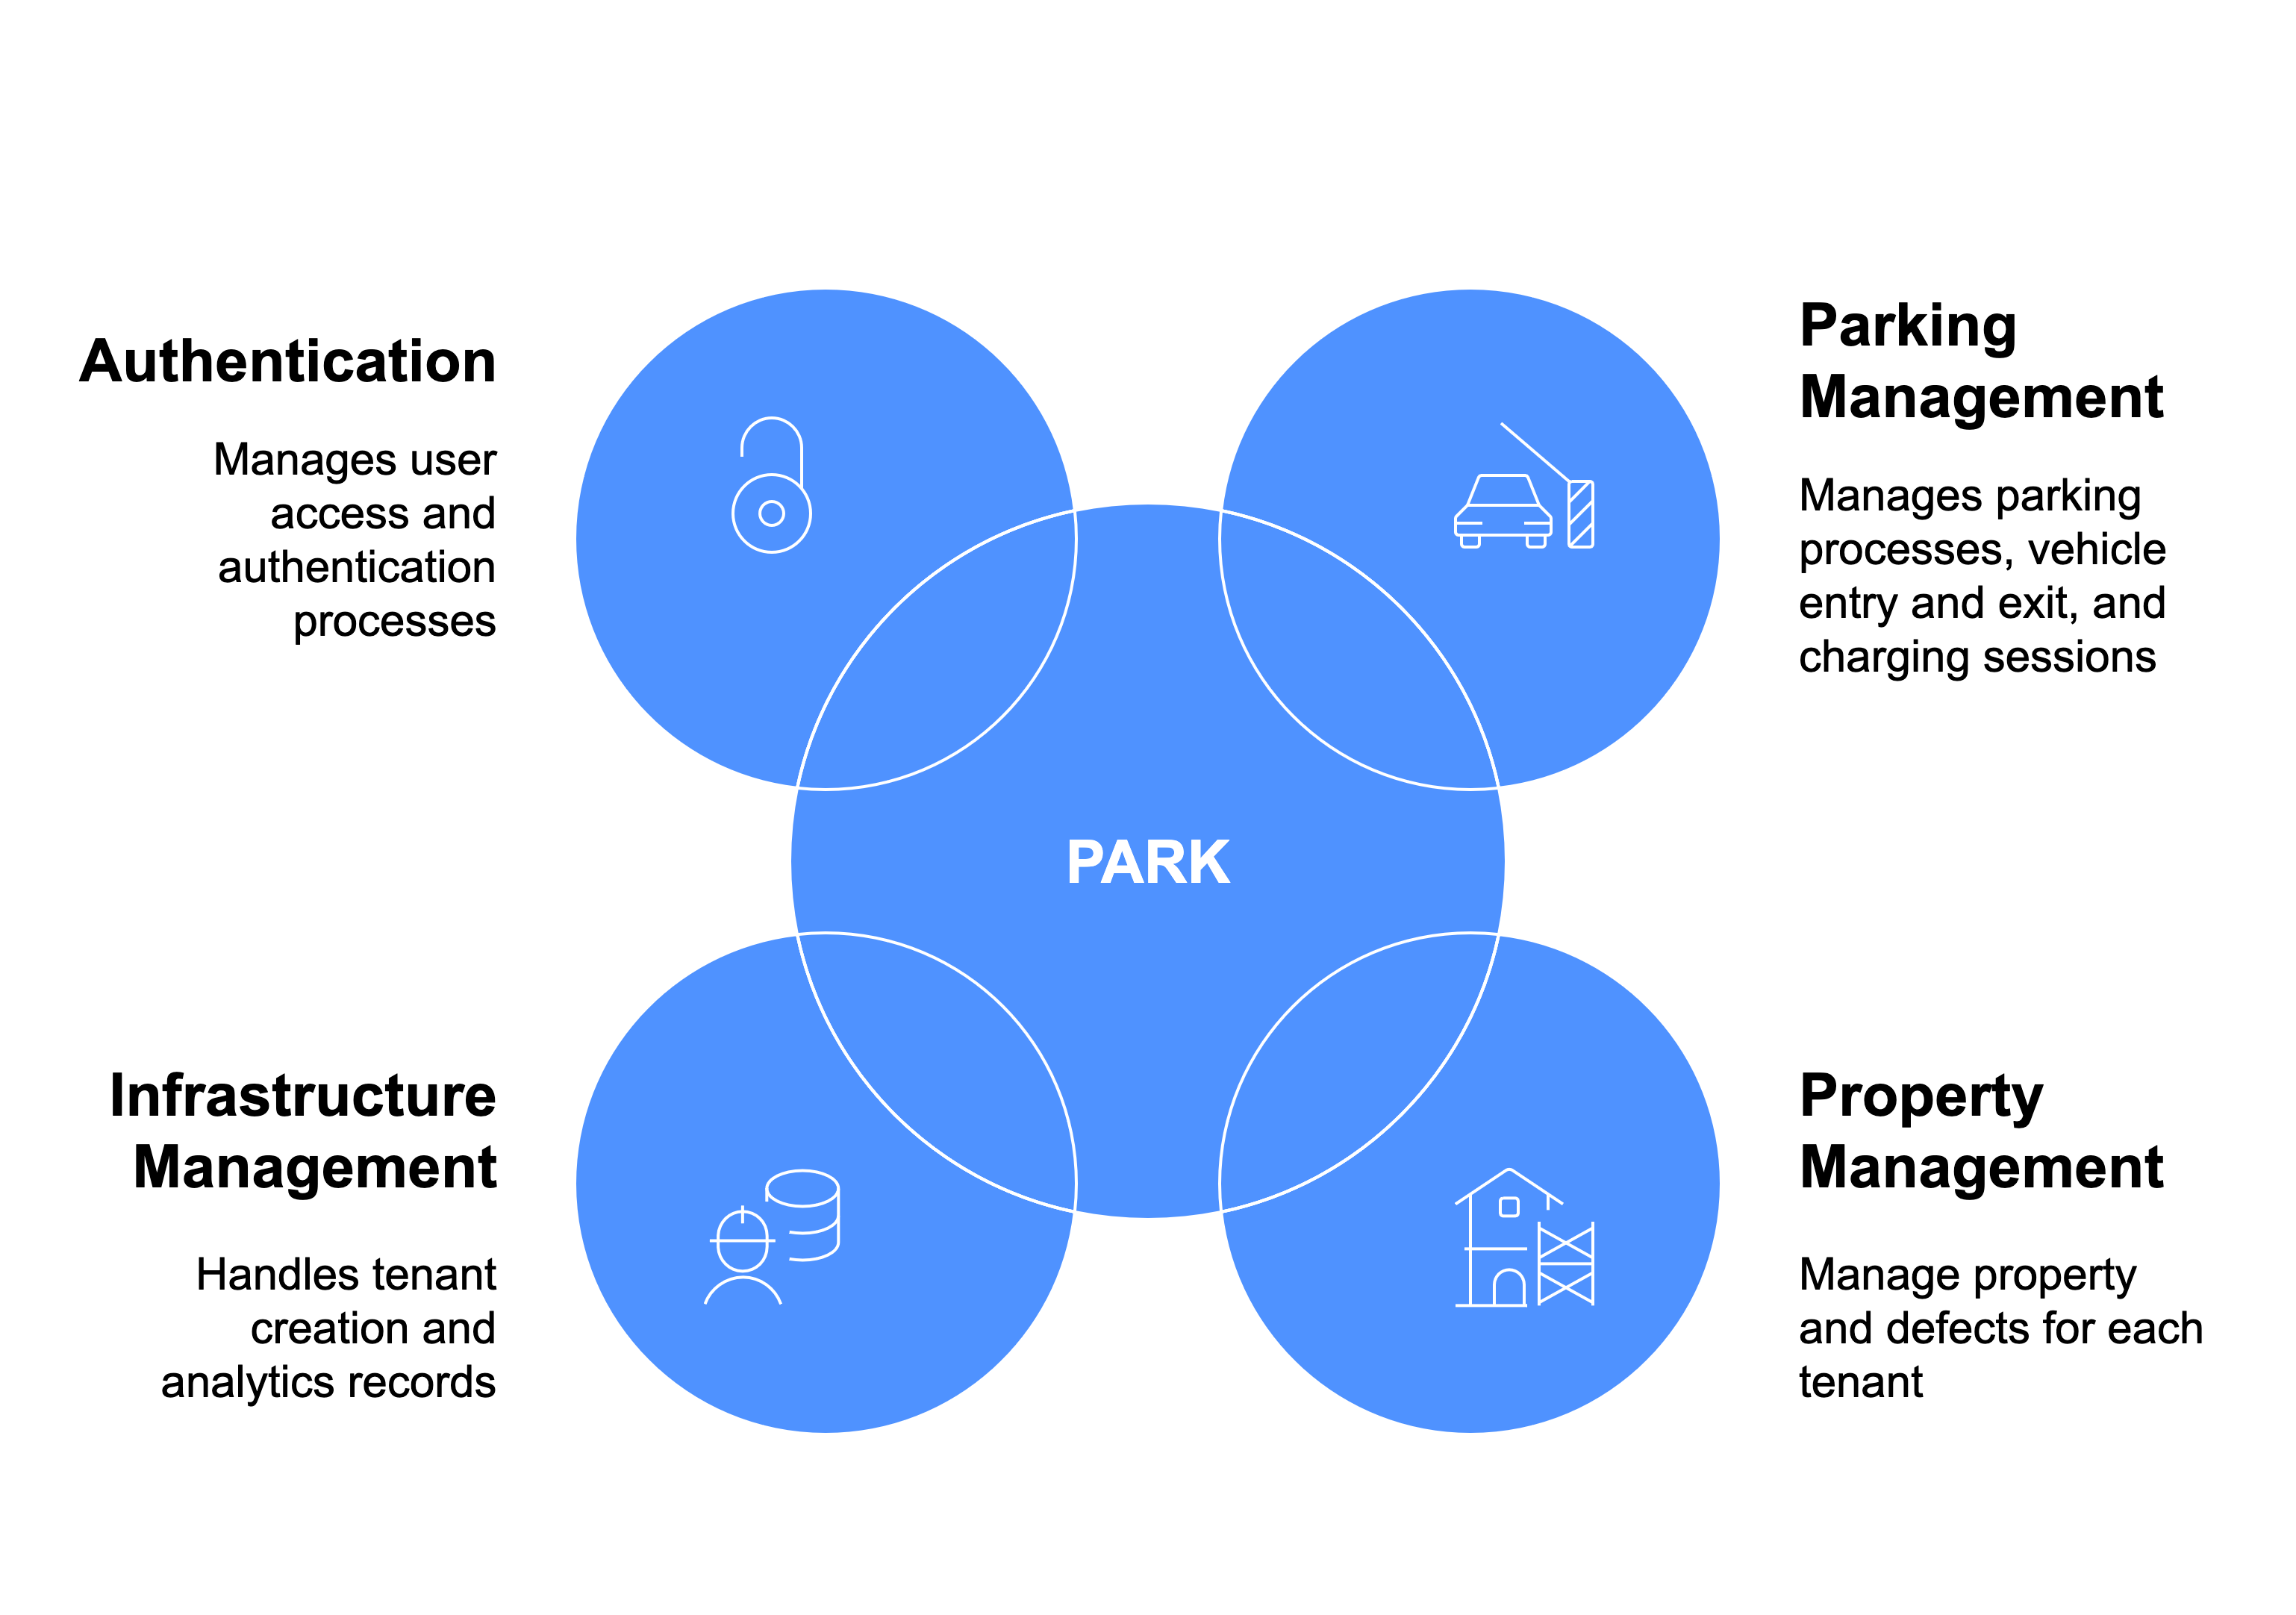
\includegraphics[width=0.9\textwidth]{resources/api-overview-blue.png}
    \caption{Übersicht der APIs}
    \label{fig:api-overview}
\end{figure}

\textbf{Parking Management:}
\begin{itemize}[noitemsep]
    \item[] \verb|GET garage|
    \item[] \verb|POST garage|
    \item[] \verb|PUT update garage|
    \item[] \verb|DELETE garage|
    \item[] \verb|GET parking occupancy|
    \item[] \verb|GET charging occupancy|
    \item[] \verb|POST car entry|
    \item[] \verb|POST handle payment|
    \item[] \verb|GET may exit|
    \item[] \verb|POST car exit|
    \item[] \verb|POST start charging session|
    \item[] \verb|POST end charging session|
    \item[] \verb|GET charging session|
    \item[] \verb|GET charging invoice|
\end{itemize}

\textbf{Property Management:}
\begin{itemize}[noitemsep]
    \item[] \verb|GET defect(s)|
    \item[] \verb|POST defect|
    \item[] \verb|DELETE defect|
    \item[] \verb|GET signed image download url|
    \item[] \verb|GET signed image upload url|
\end{itemize}

\textbf{Infrastructure Management:}
\begin{itemize}[noitemsep]
    \item[] \verb|POST add tenant|
    \item[] \verb|PUT parking occupancy record|
    \item[] \verb|GET parking occupancy record(s)|
    \item[] \verb|PUT charging occupancy record|
    \item[] \verb|GET charging occupancy record(s)|
    \item[] \verb|PUT parking duration record|
    \item[] \verb|GET parking duration record(s)|
    \item[] \verb|PUT power consumed record|
    \item[] \verb|GET power consumed record(s)|
    \item[] \verb|PUT turnover record|
    \item[] \verb|GET turnover record(s)|
    \item[] \verb|PUT defect status record|
    \item[] \verb|GET defect status record(s)|
    \item[] \verb|PUT increase request count|
    \item[] \verb|GET request count|
\end{itemize}

\textbf{Authentication:}
\begin{itemize}[noitemsep]
    \item[] \verb|GET user|
    \item[] \verb|GET all users|
    \item[] \verb|PUT update user|
    \item[] \verb|POST user|
    \item[] \verb|POST add tenant|
\end{itemize}
